\documentclass[a4paper]{article}
\def\DOCTITLE{CSC3423 Biocomputing}
% Set document attributes
\title{\DOCTITLE}

\usepackage{fullpage}
\usepackage{scrextend}
\usepackage{titlesec}
\usepackage{fancyhdr}
\usepackage{amsmath}
\usepackage{amssymb}

% Handle graphics correctly
\ifx\pdftexversion\undefined
\usepackage{graphicx}
% \usepackage[dvips]{graphicx}
\else
\usepackage[pdftex]{graphicx}
\DeclareGraphicsRule{*}{mps}{*}{}
\fi

% Setup headers and footers
\pagestyle{fancy}
\lhead{}
\chead{\DOCTITLE}
\rhead{}
\rfoot{}
\cfoot{\thepage}
\lfoot{}

% New page for each section
% \newcommand{\sectionbreak}{\clearpage}

% Set header and footer sizes
\renewcommand{\headrulewidth}{0.4pt}
\renewcommand{\footrulewidth}{0.4pt}
\setlength{\headheight}{15.2pt}
\setlength{\headsep}{15.2pt}

\setlength{\parskip}{5pt plus 1pt minus 1pt}
\setlength{\parindent}{0pt}

\newcommand{\Forall}{\;\forall\;}
\newcommand{\Mod}{\: mod \:}


\begin{document}

\tableofcontents

\section{Overview}
\label{sec:overview}

\begin{table}[h]
  \centering
  \begin{tabular}{@{}l|cccccc@{}}
    \toprule
    Problem Type     & GA/GP/MA     & NN          & ACO           & PSO         & CA          & MC          \\
    \midrule
    Optimisation     & \checkmark   &             & (\checkmark)  & \checkmark  &             &             \\
    Machine Learning & \checkmark   & \checkmark  & (\checkmark)  & \checkmark  &             &             \\
    Control          & \checkmark   & \checkmark  & (\checkmark)  & \checkmark  &             &             \\
    Simulation       & (\checkmark) &             &               &             & \checkmark  & \checkmark  \\
    \bottomrule
  \end{tabular}
  \caption{Suitability of algorithms to problems}
  \label{tab:suitability}
\end{table}

\begin{description}
  \item[GA]   Genetic Algorithm
  \item[GP]   Genetic Programming
  \item[MA]   Memetic Algorithm
  \item[NN]   Neural Network
  \item[ACO]  Ant Colony Optimisation
  \item[PSO]  Particle Swarm Optimisation
  \item[CA]   Cellular Automata
  \item[MC]   Membrane Computing
\end{description}

\section{Genetic Algorithms}
\label{sec:ga}

\subsection{Biological Inspiration}

\Para{Natural selection}

Principle that every slight change in a trait that is beneficial is preserved.

Individuals that have traits that allow them to be better adapted to the
environment are more likely to reproduce, traits are then passed to later
generations.

\Para{Genetics}

Candidate solutions to a problem represented in a chromosome composed of several
genes.

Genes are passed from generation to generation with small changes (mutations).

\subsection{Overview}

\begin{figure}[h!]
  \centering
  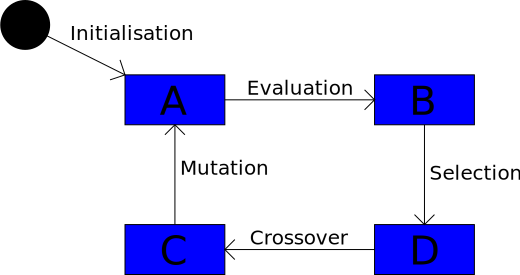
\includegraphics[width=0.5\textwidth]{out/ga_workflow.eps}
  \caption{Genetic Algorithm Workflow}
  \label{fig:ga_workflow}
\end{figure}
\FloatBarrier

\Para{Pseudocode}

\begin{listing}[h]
  \begin{minted}{python}
    population = init_random_population()
    iteration = 0
    while iteration < num_interations:
      evaluate(population)
      population = selection(population)
      population = crossover(population)
      population = mutation(population)
      iteration++
    best = get_best_individual(population)
    return best
  \end{minted}
  \caption{Genetic algorithm pseudocode}
  \label{listing:ga_pseudocode}
\end{listing}

\subsection{Population}

\begin{itemize}
  \item Set of possible solutions to the problem
  \item Most often a set (chromosome) of variables (genes)
  \item Initial population created at random
\end{itemize}

\subsection{Evaluation}

\begin{itemize}
  \item Giving a "goodness" value to each candidate solution
  \item Uses a fitness function which takes a candidate solution and determines
        how well it solves the problem
\end{itemize}

\subsection{Selection}

\begin{itemize}
  \item Choosing individuals to be in the next population
  \item Rewards best individuals (i.e. those with the best fitness values)
\end{itemize}

\subsubsection{Roulette Wheel Selection}

\begin{itemize}
  \item Probability of selection is proportional to fitness of individual
  \item Make as many selections (spins of wheel) as individuals to be selected
  \item Individuals may be selected multiple times
\end{itemize}

\begin{figure}[h!]
  \centering
  \includegraphics[width=0.4\textwidth]{out/roulette_wheel_selection.eps}
  \caption{Roulette Wheel Selection}
  \label{fig:roulette_wheel_selection}
\end{figure}
\FloatBarrier

\subsubsection{Stochastic Universal Sampling}

\begin{itemize}
  \item Similar to Roulette Wheel Selection
  \item Do one spin but divide "pointer" into as many individuals to be selected
\end{itemize}

\begin{figure}[h!]
  \centering
  \includegraphics[width=0.4\textwidth]{out/stochastic_universal_sampling.eps}
  \caption{Stochastic Universal Sampling}
  \label{fig:stochastic_universal_sampling}
\end{figure}
\FloatBarrier

\subsubsection{Tournament Selection}

\begin{itemize}
  \item Select the best individual from a randomly selected subset of the
        population
\end{itemize}

\begin{listing}[h]
  \begin{minted}{python}
    new_population = []
    while population.size() > 0:
      tournament = select_random_subset(population, tournament_size)
      tournament = sort_by_fitness(tournament)
      new_population.add(tournament[0])
    return new_population
  \end{minted}
  \caption{Tournament selection pseudocode}
  \label{listing:ga_tournament_selection_pseudocode}
\end{listing}

\subsubsection{Truncation Selection}

\begin{itemize}
  \item Keep only the best $n$ individuals in a population
\end{itemize}

\subsubsection{Comparison of selection methods}

\begin{description}
  \item[Roulette Wheel \& Stochastic Selection] \hfill \\
    \begin{itemize}
      \item Fitness proportionate
      \item Chance of being selected is proportionate to fitness value
      \item Selection becomes random when fitness values are close (e.g. in
            later GA iterations)
    \end{itemize}

  \item[Tournament \& Truncation Selection] \hfill \\
    \begin{itemize}
      \item Rank based
      \item Best individual will always win a tournament
      \item More stable selection pressure
    \end{itemize}

\end{description}

\subsection{Crossover}

\begin{itemize}
  \item Exchanging genes between two individuals
  \item Takes two individuals from the population and generates two offspring
  \item e.g. For a bit array, one offspring takes first section of array and
        second of another, and vice-versa
  \item e.g. For numerical genes the blend alpha operator picks a random value
        between the two parent genes
\end{itemize}

\subsection{Mutation}

\begin{itemize}
  \item Making small/subtle modifications to an individual
  \item Probability $P_{m}$ of mutation can be set either per chromosome or per
        individual
  \item e.g. Randomly flipping a bit where the chromosome is a bit array
  \item e.g. Adding a random value to a numerical gene
\end{itemize}

\subsection{Replacement}

\begin{itemize}
  \item Alternative to generational genetic algorithm
  \item Steady state genetic algorithm
    \begin{itemize}
      \item Elitism
      \item Selection chooses two parents who produce two offspring
      \item Offspring are inserted into the parent population, replacing the
            two individuals with lowest fitness
    \end{itemize}
\end{itemize}

\subsection{Knowledge Representation}

Nominal attributes:

\begin{itemize}
  \item Set of rules and logic predicates
\end{itemize}

Real valued attributes:

\begin{itemize}
  \item Hyperrectangle ($n$ dimension rectangle)
  \item Hyperellipsoid ($n$ dimension circle)
  \item Decision trees
  \item Synthetic prototypes (e.g. nearest neighbour)
  \item Linear classifier (separate instances of classes for classification
        problems)
\end{itemize}

\begin{figure}[h]
  \centering
  \begin{subfigure}[b]{0.4\textwidth}
    \includegraphics[width=\textwidth]{out/kr_decision_tree.eps}
    \caption{Decision Tree}
  \end{subfigure}
  \begin{subfigure}[b]{0.4\textwidth}
    \includegraphics[width=\textwidth]{out/kr_nearest_neighbour.eps}
    \caption{Nearest Neighbour}
  \end{subfigure}
  \caption{}
  \label{fig:ga_knowledge_representations}
\end{figure}
\FloatBarrier

\subsection{Tuning}

\begin{itemize}
  \item Required to ensure a proper evolutionary process
  \item GA learns well when exploration and exploitation are balanced
    \begin{description}
      \item[Exploration]
        Directing population to unknown areas of the problem space
      \item[Exploitation]
        Directing the population to most promising (based on fitness) parts of
        the problem space
    \end{description}
  \item Too much exploitation can lead to convergence to a sub-optimal solution
        (premature convergence)
    \begin{itemize}
      \item If population is too similar then crossover operator no longer
            provides effective exploration
    \end{itemize}
  \item Too much exploration risks:
    \begin{itemize}
      \item Slowing down the learning process
      \item If probabilities are too high then crossover and mutation may harm
            the overall population fitness
    \end{itemize}
  \item Innovation time $t_{i}$ is the average time taken to create an
        individual with better fitness than the current best individual
\end{itemize}

\subsection{Machine Learning}

\begin{description}
  \item[Supevised learning] \hfill \\
    \begin{itemize}
      \item Learning to solve a problem
      \item If output is discrete \RArrow Classification (output value known as
            a class)
      \item If output is continuous \RArrow Regression
      \item Use a training set to train the genetic algorithm and a testing set
            to verify the generated model
      \item Optimise initialisation by creating initial population based on
            training data
    \end{itemize}

  \item[Unsupervised learning] \hfill \\
    \begin{itemize}
      \item Identifying patters/clusters
    \end{itemize}

\end{description}

\subsection{Parallel Genetic Algorithms}

\begin{itemize}
  \item Genetic algorithms tend to be slow
  \item Majority of genetic operations can be parallelised (all but crossover)
  \item Several systems exist for this:
    \begin{description}
      \item[Master-Slave model]
        GA cycle is is run on master, slaves perform operations
      \item[Island Model]
        Population is divided across nodes
      \item[Cellular GA]
        Population distributed across 2D lattice
    \end{description}
\end{itemize}

\section{Genetic Programming}
\label{sec:gp}

\begin{itemize}
  \item Very similar concept to Genetic Algorithms \ref{sec:ga}
  \item Instead of evolving a solution, evolve a program

\end{itemize}

\subsection{Program Representation}

\begin{itemize}
  \item Classic method is to represent programs as a tree representing a
        formula
  \item Modern methods can also create other representations
    \begin{itemize}
      \item e.g. Cartesian Genetic Programming creates graphs
    \end{itemize}
  \item Internal nodes of tree are functions/operations
  \item Leaves are either variables/parameters or constants
    \begin{itemize}
      \item Constants can be predefined or assigned a random value within a
            predefined range
    \end{itemize}
\end{itemize}

\Para{Example}

Figure \ref{fig:gp_tree_example} shows a tree representing the equation:
\[
  \frac{4 + P3}{P1 - sin(P2)}
\]

\begin{figure}[h!]
  \centering
  \includegraphics[width=0.3\textwidth]{out/gp_tree_example.eps}
  \caption{Example Tree}
  \label{fig:gp_tree_example}
\end{figure}
\FloatBarrier

\subsection{Initialisation}

\begin{itemize}
  \item Initial tree is generated randomly
  \item Maximum depth of tree is predefined
  \item Strategies for generation:
    \begin{description}
      \item[Grow] \hfill \\
        Generate a tree at random with leaves up to the maximum depth
      \item[Fill] \hfill \\
        Generate a tree at random with all leaves at the maximum depth
      \item[Hybrid] \hfill \\
        For each level of depth, initialise a uniform number of trees, half of
        which using Grow and half using Full
    \end{description}
\end{itemize}

\begin{figure}[h]
  \centering
  \begin{subfigure}[t!]{0.4\textwidth}
    \includegraphics[width=0.5\textwidth]{out/gp_tree_grow.eps}
    \caption{Grow}
  \end{subfigure}
  \begin{subfigure}[t!]{0.4\textwidth}
    \includegraphics[width=0.8\textwidth]{out/gp_tree_fill.eps}
    \caption{Fill}
  \end{subfigure}
  \caption{Tree initialisation}
  \label{fig:gp_initialisation}
\end{figure}
\FloatBarrier

\subsection{Evaluation/Execution}

\begin{itemize}
  \item Evaluation is done by averaging error over all test cases, giving a
        fitness value
  \item Recursive execution is easy but inefficient
  \item Converting a tree to Reverse Polish Notation solves problem
\end{itemize}

\begin{listing}[h]
  \begin{minted}{text}
    for each element e:
      if e is value:
        push e to the stack
      else if e is operator:
        pop as many elements from the stack as the operator has parameters
        execute the operator
        push the result to the stack
    return value at top of stack
  \end{minted}
  \caption{Genetic programming execution pseudocode}
  \label{listing:gp_eval_pseudocode}
\end{listing}

\subsection{Crossover}

Exchange subtrees between parents.

\Para{Example}

\begin{figure}[h]
  \centering
  \begin{subfigure}[t!]{0.4\textwidth}
    \includegraphics[width=0.8\textwidth]{out/gp_tree_example.eps}
  \end{subfigure}
  \begin{subfigure}[t!]{0.4\textwidth}
    \includegraphics[width=0.8\textwidth]{out/gp_tree_example_mutation.eps}
  \end{subfigure}
  \caption{Tree crossover parents}
  \label{fig:gp_crossover_parents}
\end{figure}
\FloatBarrier

\begin{figure}[h]
  \centering
  \begin{subfigure}[t!]{0.4\textwidth}
    \includegraphics[width=0.8\textwidth]{out/gp_tree_child_1.eps}
  \end{subfigure}
  \begin{subfigure}[t!]{0.4\textwidth}
    \includegraphics[width=0.8\textwidth]{out/gp_tree_child_2.eps}
  \end{subfigure}
  \caption{Tree crossover children}
  \label{fig:gp_crossover_children}
\end{figure}
\FloatBarrier

\subsection{Mutation}

Replace entire subtrees with a randomly generated subtree.

\Para{Example}

\begin{figure}[h]
  \centering
  \begin{subfigure}[t!]{0.4\textwidth}
    \includegraphics[width=0.8\textwidth]{out/gp_tree_example.eps}
    \caption{Before}
  \end{subfigure}
  \begin{subfigure}[t!]{0.4\textwidth}
    \includegraphics[width=0.8\textwidth]{out/gp_tree_example_mutation.eps}
    \caption{After}
  \end{subfigure}
  \caption{Tree mutation}
  \label{fig:gp_mutation}
\end{figure}
\FloatBarrier

\subsection{Bloat}

\begin{itemize}
  \item Growth of program tree without improvement in fitness
  \item Bloat can affect any evolutionary paradigm where the representation
        has variable length
  \item Solutions:
    \begin{description}
      \item[Restrict tree depth] \hfill \\
        May affect evolutionary process making it unable to find a good
        solution
      \item[Simplification] \hfill \\
        Very difficult to do efficiently
      \item[Add fitness penalty to large trees] \hfill \\
        Smaller fitness for solutions with larger trees
      \item[Consider tree size in selection] \hfill \\
        When two individuals have equal fitness, prefer the smaller tree
    \end{description}
\end{itemize}

\subsection{Applications}

\begin{description}
  \item[Regression] \hfill \\
    Reverse engineering a mathematical formula given a dataset of output values
    for given input values.

    This gives an approximation of the original formula that created the
    dataset.

  \item[Generating Electronic Circuits] \hfill \\
    Tree topology defines schematic.

    Leaves define component values (inductance, capacitance, etc.).

  \item[Control] \hfill \\
    Optimising gains of a PID controller.

  \item[Puzzle Solvers] \hfill \\
    e.g. FreeCell solver using hybrid genetic algorithm and genetic
    programming.

  \item[Generation of Audio Synhesizers] \hfill \\
    Using Cartesian Generic Programming to generate a graph structure.

\end{description}

\section{Neural Networks}
\label{sec:nn}

TODO

\section{Memetic Algorithms}
\label{sec:ma}

TODO

\section{Swarm Intelligence}
\label{sec:swarm}

TODO

\section{Cellular Automata}
\label{sec:ca}

TODO

\section{Membrane Computing}
\label{sec:membrane}

TODO

\section{DNA Computing}
\label{sec:dna}

TODO

\end{document}
